\documentclass[english]{beamer}\usepackage[]{graphicx}\usepackage[]{xcolor}
% maxwidth is the original width if it is less than linewidth
% otherwise use linewidth (to make sure the graphics do not exceed the margin)
\makeatletter
\def\maxwidth{ %
  \ifdim\Gin@nat@width>\linewidth
    \linewidth
  \else
    \Gin@nat@width
  \fi
}
\makeatother

\definecolor{fgcolor}{rgb}{0.345, 0.345, 0.345}
\newcommand{\hlnum}[1]{\textcolor[rgb]{0.686,0.059,0.569}{#1}}%
\newcommand{\hlstr}[1]{\textcolor[rgb]{0.192,0.494,0.8}{#1}}%
\newcommand{\hlcom}[1]{\textcolor[rgb]{0.678,0.584,0.686}{\textit{#1}}}%
\newcommand{\hlopt}[1]{\textcolor[rgb]{0,0,0}{#1}}%
\newcommand{\hlstd}[1]{\textcolor[rgb]{0.345,0.345,0.345}{#1}}%
\newcommand{\hlkwa}[1]{\textcolor[rgb]{0.161,0.373,0.58}{\textbf{#1}}}%
\newcommand{\hlkwb}[1]{\textcolor[rgb]{0.69,0.353,0.396}{#1}}%
\newcommand{\hlkwc}[1]{\textcolor[rgb]{0.333,0.667,0.333}{#1}}%
\newcommand{\hlkwd}[1]{\textcolor[rgb]{0.737,0.353,0.396}{\textbf{#1}}}%
\let\hlipl\hlkwb

\usepackage{framed}
\makeatletter
\newenvironment{kframe}{%
 \def\at@end@of@kframe{}%
 \ifinner\ifhmode%
  \def\at@end@of@kframe{\end{minipage}}%
  \begin{minipage}{\columnwidth}%
 \fi\fi%
 \def\FrameCommand##1{\hskip\@totalleftmargin \hskip-\fboxsep
 \colorbox{shadecolor}{##1}\hskip-\fboxsep
     % There is no \\@totalrightmargin, so:
     \hskip-\linewidth \hskip-\@totalleftmargin \hskip\columnwidth}%
 \MakeFramed {\advance\hsize-\width
   \@totalleftmargin\z@ \linewidth\hsize
   \@setminipage}}%
 {\par\unskip\endMakeFramed%
 \at@end@of@kframe}
\makeatother

\definecolor{shadecolor}{rgb}{.97, .97, .97}
\definecolor{messagecolor}{rgb}{0, 0, 0}
\definecolor{warningcolor}{rgb}{1, 0, 1}
\definecolor{errorcolor}{rgb}{1, 0, 0}
\newenvironment{knitrout}{}{} % an empty environment to be redefined in TeX

\usepackage{alltt}

%% The most common packages are already included in:
\usetheme{biostat}
\usepackage{xcolor}
\usepackage{hyperref}

%% Custom color for links (biostat blue)
\definecolor{mylinkcolor}{RGB}{0,40,165}

\hypersetup{
  colorlinks=true,
  urlcolor = mylinkcolor,
  linkcolor=mylinkcolor,
  urlcolor=mylinkcolor,
  citecolor=mylinkcolor,
  filecolor = mylinkcolor
}

%%%%%%%%%%%%%%%%%%%%%%%%%%%%%%%%%%%%%%%%%%%%%%%%%%%%%%%%

%% Header data: (adjust to your needs:
\def\uzhunit{STA421 Foundations of Bayesian Methodology}             %% if (not) needed comment/uncomment
%\def\uzhunitext{STA480}

\title[Monte Carlo method]{History of the Monte Carlo method}
%% Optional Argument in [Brackets]: Short Title for Footline

%% The following are all optional, simply comment them
\subtitle{\textbf{Big picture contribution}}
%%\institute{STA480 Statistical consulting}  %% optional
\author{Group 2: Jan Hohenheim, Holly Vuarnoz, Sophie Haldemann,
Andrea Staub, Emanuel Mauch}
\date{\today}

%%%%%%%%%%%%%%%%%%%%%%%%%%%%%%%%%%%%%%%%%%%%%%%%%%%%%%%%


%%%%%%%%%%%%%%%%%%%%%%%%%%%%%%%%%%%%%%%%%%%%%%%%%%%%%%%%

\IfFileExists{upquote.sty}{\usepackage{upquote}}{}
\begin{document}
\maketitle


%%%%%%%%%%%%%%%%%%%%%%%%%%%%%%%%%%%%%%%%%%%%%%%%%%%%%%%%
%% Introduction
%%%%%%%%%%%%%%%%%%%%%%%%%%%%%%%%%%%%%%%%%%%%%%%%%%%%%%%%
\begin{frame}{The History}

\begin{itemize}\setlength\itemsep{1em} % Increase spacing here
    \item Revolutionary idea of Comte de Buffon (1707-1788):
    \begin{itemize}
      \item Using randomness in a deterministic way
      \item Buffon's Needle for calculating Pi (\(\pi\)) 
    \end{itemize}
    \item 1940s Los Alamos, World War II:
    \begin{itemize}
      \item Simulations for nuclear weapons research
      \item Named after Monte Carlo Casino in Monaco
    \end{itemize}
\end{itemize}

\end{frame}


%%%%%%%%%%%%%%%%%%%%%%%%%%%%%%%%%%%%%%%%%%%%%%%%%%%%%%%%
%% The Method
%%%%%%%%%%%%%%%%%%%%%%%%%%%%%%%%%%%%%%%%%%%%%%%%%%%%%%%%
\begin{frame}{The Method}

Many simulations follow this pattern:
\begin{itemize}
  \item Model system with probability density functions (PDFs)
  \item Sample repeatedly from PDFs
  \item Compute statistics of interest
\end{itemize}

Requirement: \textbf{exact object is known}\\
$\rightarrow$ e.g. finance, physics and engineering
\end{frame}



\begin{frame}{Marble Example: Estimating Pi (\(\pi\))}

\begin{figure}
  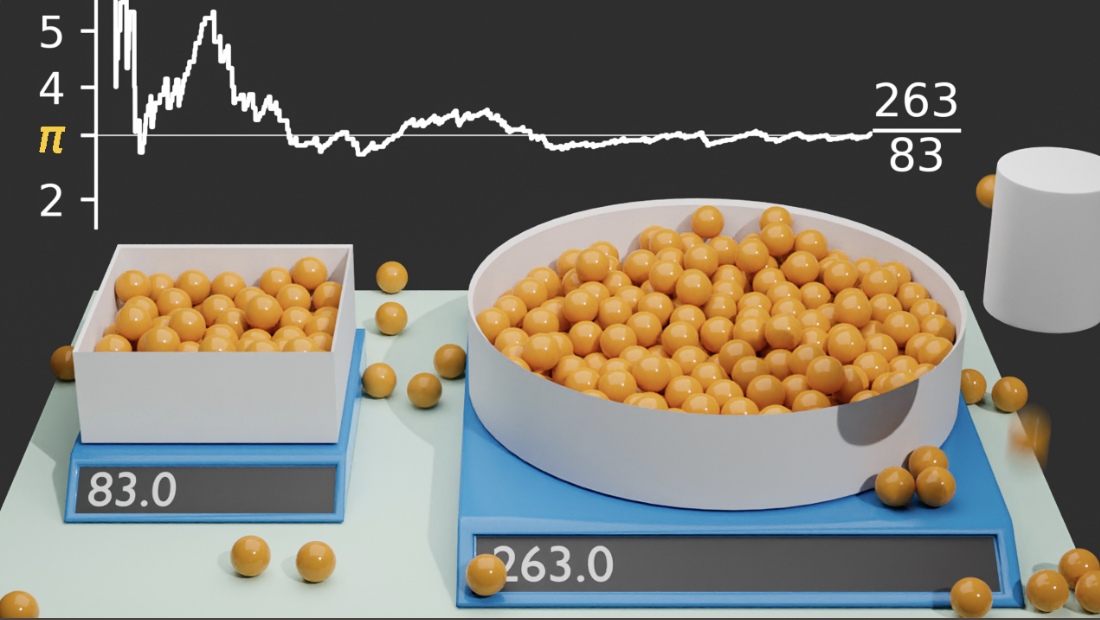
\includegraphics[width=0.45\textwidth]{marble}
  \hspace{0.5cm} % Spacing between the images
  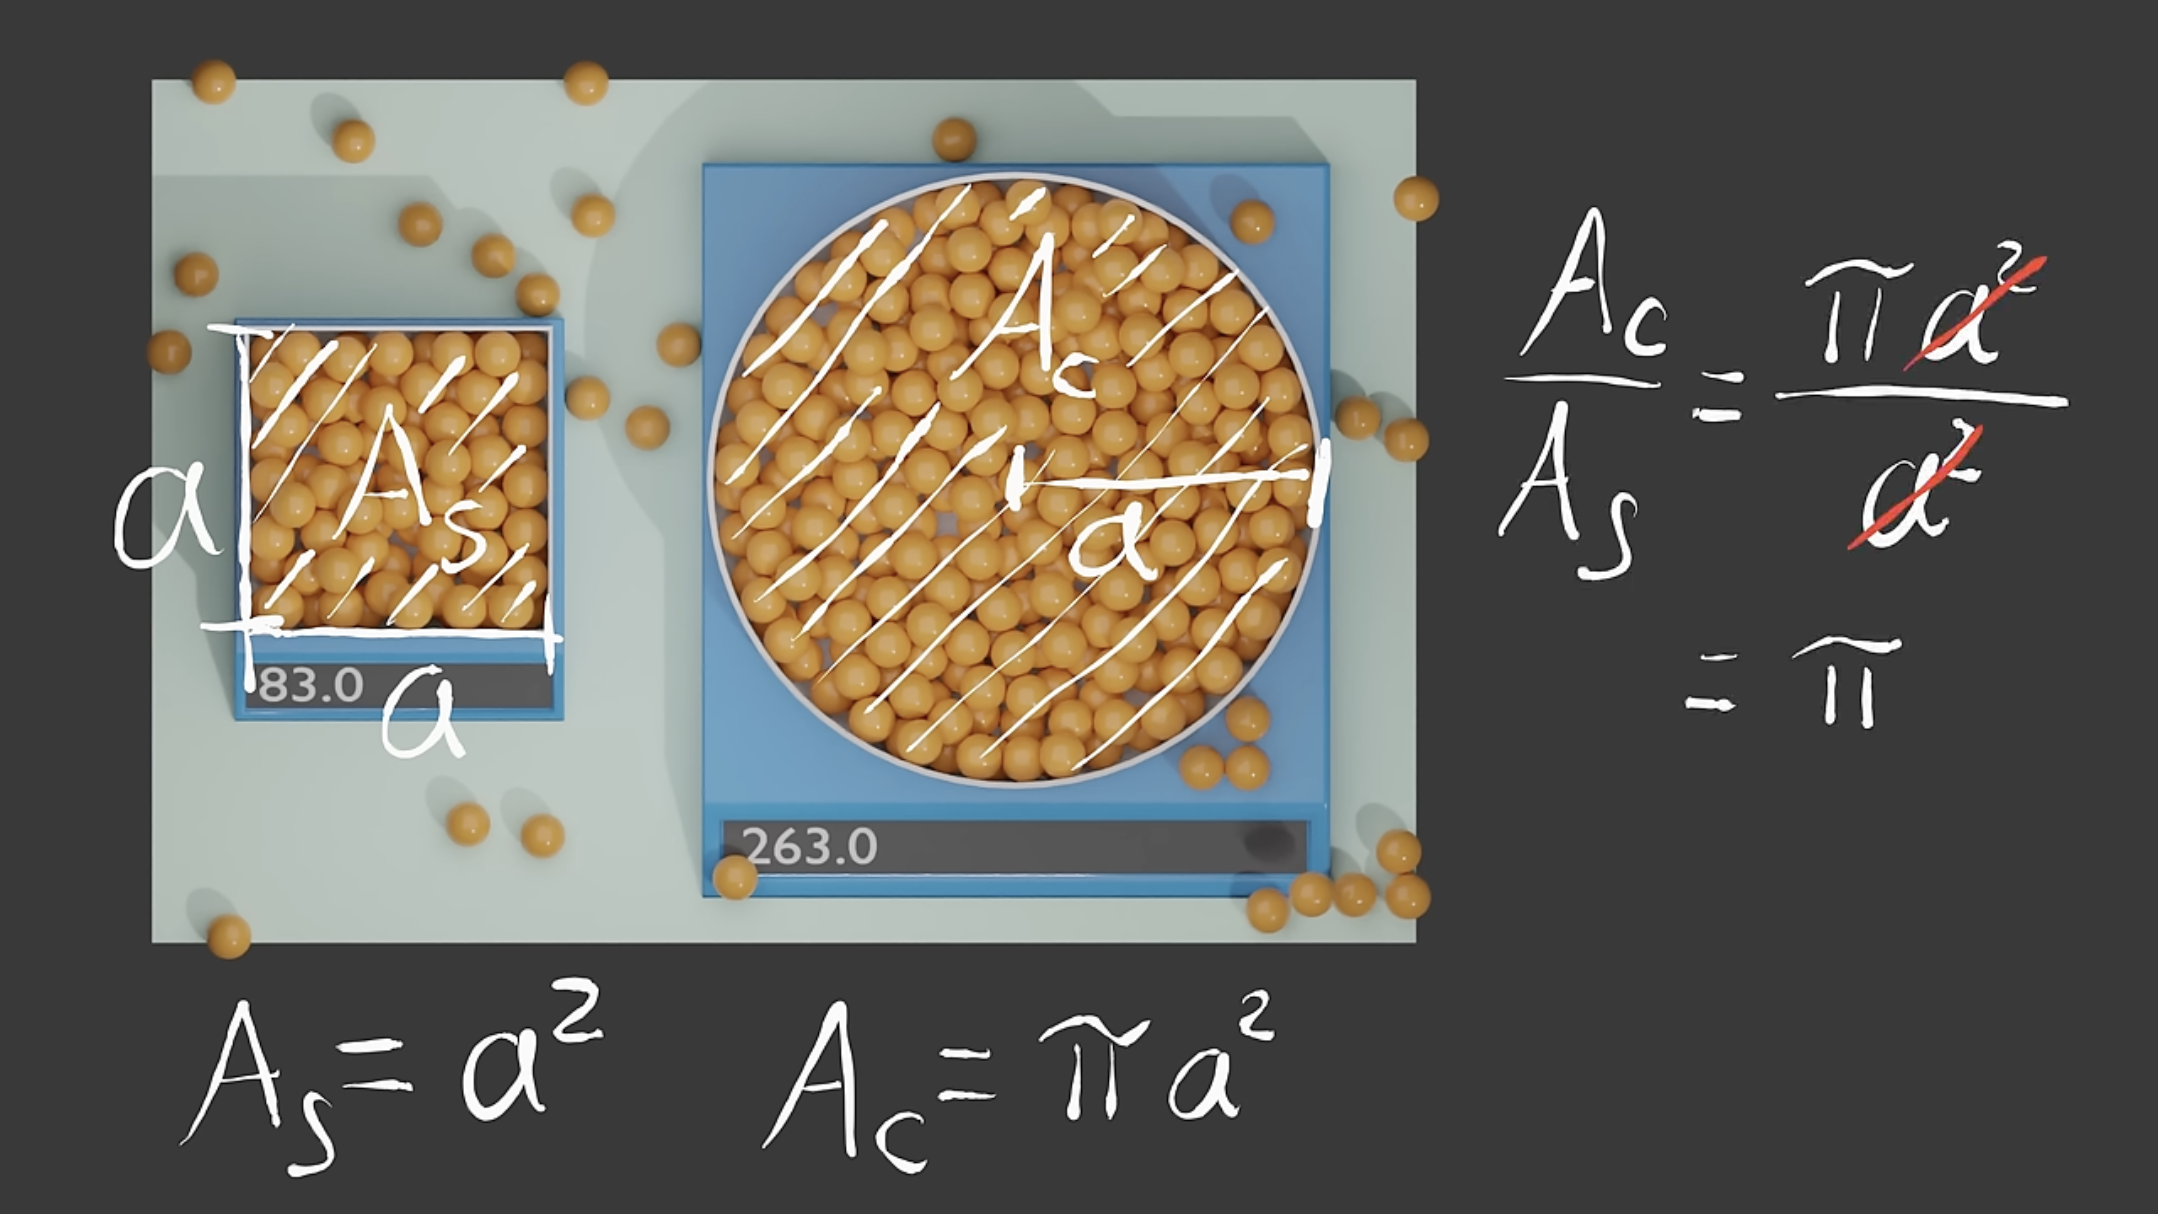
\includegraphics[width=0.45\textwidth]{marble2}
  \caption{The number Pi is determined by randomly dropping marbles into two bowls. Proportion of marbles ending up in the two bowls approaches \(\pi\) as the simulation progresses. See \href{https://www.youtube.com/watch?v=7ESK5SaP-bc}{YouTube video}.}
\end{figure}
\end{frame}

\begin{frame}{Law of Large Numbers}
Let \((X_1, \ldots, X_n)\) be a sequence of independent and identically distributed (i.i.d.) random variables with finite expectation \(\mu\). Then, as \(n \rightarrow \infty\),

\[
\frac{1}{n} \sum_{i=1}^{n} X_i \overset{P}{\rightarrow} \mu
\]

\cite{held2014}.


\end{frame}



\begin{frame}{Inverse Transform Sampling: Generating Samples}

\begin{itemize}
  \item Generate i.i.d. samples from uniform distribution [0, 1]
  \item Inverse transform sampling:
    \begin{itemize}
        \item Apply inverse CDF to transform uniform samples to target distribution
        \item Works because \(P[F^{-1}(U) \leq x] = P[U \leq F(x)] = F(x)\)
    \end{itemize}
  \item Example: Exponential distribution
    \begin{itemize}
        \item For \(F(x) = 1 - \exp(-\lambda x), x \geq 0\),
        \item Set \(1 - \exp(-\lambda x) = u\),
        \item Solve for \(x\): \(x = -\frac{1}{\lambda} \log(1 - u)\)
    \end{itemize}
  \item Enables sampling from any distribution with known inverse CDF
\end{itemize}

\end{frame}



%%%%%%%%%%%%%%%%%%%%%%%%%%%%%%%%%%%%%%%%%%%%%%%%%%%%%%%%
%% Example from Worksheet 1
%%%%%%%%%%%%%%%%%%%%%%%%%%%%%%%%%%%%%%%%%%%%%%%%%%%%%%%%




\begin{frame}[fragile]{Worksheet 1: Random Sample vs True Distribution}
Let the random variable \(X \sim N(\mu, \sigma^2)\), with \(\mu = 160\) and \(\sigma = 20\). Generate a Monte Carlo sample \(Xs\) of size \(M = 1000\).

\begin{knitrout}\small
\begin{knitrout}
\definecolor{shadecolor}{rgb}{0.969, 0.969, 0.969}\color{fgcolor}\begin{kframe}
\begin{alltt}
\hlstd{M} \hlkwb{<-} \hlnum{1000}
\hlstd{mu} \hlkwb{<-} \hlnum{160}
\hlstd{sigma} \hlkwb{<-} \hlnum{20}
\hlkwd{set.seed}\hlstd{(}\hlnum{44566}\hlstd{)}
\hlstd{Xs} \hlkwb{<-} \hlkwd{rnorm}\hlstd{(}\hlkwc{n} \hlstd{= M,} \hlkwc{mean} \hlstd{= mu,} \hlkwc{sd} \hlstd{= sigma)}
\end{alltt}
\end{kframe}
\end{knitrout}
\end{knitrout}
\end{frame}




\begin{frame}[fragile]
\begin{knitrout}
\definecolor{shadecolor}{rgb}{0.969, 0.969, 0.969}\color{fgcolor}

{\centering 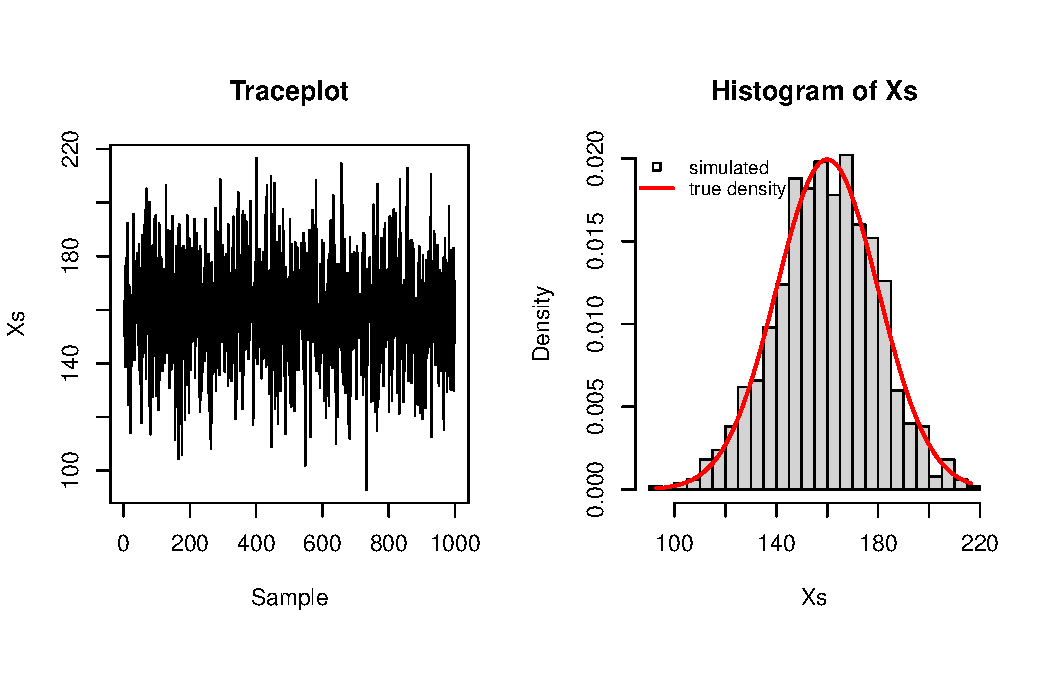
\includegraphics[width=\maxwidth]{figures/figpart3-1} 

}


\end{knitrout}
\end{frame}


\begin{frame}{Take Home Message}
\textbf{Why we use it}: 
\begin{itemize}
\item In Bayesian analysis posteriors aren't easy to work with
\item Calculation of integrals is complex
\item Monte Carlo simulation is used to numerically solve a complex problem through repeated random sampling
\end{itemize}
\end{frame}




%%%%%%%%%%%%%%%%%%%%%%%%%%%%%%%%%%%%%%%%%%%%%%%%%%%%%%%%
\begin{frame}{Bibliography}
   \footnotesize
   \bibliographystyle{apalike}
   \nocite{held2014}
   \nocite{Harrison2010}
   \nocite{Marble2020}
\bibliography{biblio}
\end{frame}

%%%%%%%%%%%%%%%%%%%%%%%%%%%%%%%%%%%%%%%%%%%%%%%%%%%%%%%%

\end{document}
